\documentclass{UoNMCHA}
\usepackage[authoryear]{natbib}
\usepackage{array,booktabs} % For nice tables
\usepackage{amsmath,amsfonts,amssymb} % For nice maths
\usepackage{color,soul}
\usepackage{enumerate}
\usepackage{listings}
\usepackage{subcaption}
\usepackage{hyperref}
\usepackage[parfill]{parskip}   % For replacing paragraph indenting with a newline instead
\usepackage[section]{placeins}
\usepackage{graphicx}
\usepackage{float}
\graphicspath{ {./images/} }


% Number equations per section
\numberwithin{equation}{section}

\hypersetup{
%    bookmarks=true,         % show bookmarks bar?
%    unicode=false,          % non-Latin characters in AcrobatÕs bookmarks
%    pdftoolbar=true,        % show AcrobatÕs toolbar?
%    pdfmenubar=true,        % show AcrobatÕs menu?
%    pdffitwindow=false,     % window fit to page when opened
%    pdfstartview={FitH},    % fits the width of the page to the window
%    pdftitle={My title},    % title
%    pdfauthor={Author},     % author
%    pdfsubject={Subject},   % subject of the document
%    pdfcreator={Creator},   % creator of the document
%    pdfproducer={Producer}, % producer of the document
%    pdfkeywords={keyword1} {key2} {key3}, % list of keywords
%    pdfnewwindow=true,      % links in new window
    colorlinks=true,       % false: boxed links; true: colored links
    linkcolor=blue,          % color of internal links
    citecolor=blue,        % color of links to bibliography
%    filecolor=magenta,      % color of file links
    urlcolor=blue           % color of external links
}

\definecolor{MATLABKeyword}{rgb}{0,0,1}
\definecolor{MATLABComment}{rgb}{0.1328125,0.54296875,0.1328125}
\definecolor{MATLABString}{rgb}{0.625,0.125,0.9375}

\lstset{language=Matlab,
    basicstyle=\small\ttfamily,
    keywordstyle=\color{MATLABKeyword},
    %identifierstyle=,
    commentstyle=\color{MATLABComment},
    stringstyle=\color{MATLABString},
    numberstyle=\tiny,
    %numbers=left,
    basewidth=0.5em}
%%%%%%%%%%%%%%%%%%%%%%%%%%%%%%%
%%%%%%%%%%%%%%%%%%%%%%%%%%%%%%%GPT HAS EDITED THIS OG VERSION STORED AS COMMENTS
%%%%%%%%%%%%%%%%%%%%%%%%%%%%%%%
\firstpage{1} % Set page number for first page
\UoNMCHAreportNo{MECH4841 Part B} %Report number
\UoNMCHAyear{2023} % Year
\shorttitle{Automating A Field Spectrometer For Lab Use} %For odd pages
%%%%%%%%%%%%%%%%%%%%%%%%%%%%%%%%%%%%%%%%%%%%%%%%%%%%
\begin{document}
	\newpage
	\title{Design And Implement A System To Automate The Use Of A Field Spectrometer For Mass Data Collection \\ \ \\
		{\small Final Year Project Report - MECH4841 Part B  \\March 2023}}
	\author[UoNMCHA]{Michael Easdown}
	\address[UoNMCHA]{
		Student of Mechatronics Engineering,\\
		The University of Newcastle, Callaghan, NSW 2308, AUSTRALIA \\
		Student Number: 3184567 \\
		E-mail: \href{mailto:michael.easdown@uon.edu.au}{\textsf{michael.easdown@uon.edu.au}}}
%%%%%%%%%%%%%%%%%%%%%%%%%%%%%%%
\maketitle
\onecolumn
\newpage
\section*{Preamble}\label{sec:Preamble}
The following list details the use of certain terms and phrases that may not be known to the reader, in order to assist in understanding specific aspects of the report.\\
\begin{itemize}
	\item HLR: Hone Lab Red. The instrument developed by Hone Global for in-field spectroscopy.
	\item Scanning: 'Taking a scan' or 'scanning' refers to using the HLR to capture data.
	\item Background Cap: A device fitted to the face of the HLR to calibrate the sensor before scanning material.
	\item Desktop Application: A custom-built application that runs on Windows to control the HLR while scanning.
	\item Sub-sampling: The HLR does not scan the entire surface of the material being scanned. To get an accurate reading of the entire sample, a number of 'sub-samples' are taken and interpolated to give a single reading that represents the entire sample. This involves taking a number of individual scans to be combined, resulting in a scan that better captures the entire sample. This process is known as sub-sampling.
	\item System: This refers to the overall design that is to be built and tested. May also be referred to as 'final system' or 'overall system'.
	\item Sub-system: This refers to any combination of components that performs a distinct operation within the larger design/system.
	\item SDK: A firmware package that allows the instrument to be controlled with a micro-controller.
\end{itemize}
%%%%%%%%%%%%%%%%%%%%%%%%%%%%%%%%%%%
\newpage
\section*{Abstract}\label{sec:Abstract}
To be written later, keep it short
%%%%%%%%%%%%%%%%%%%%%%%%%%%%%%%%%%%
\newpage
\section*{Executive Summary}\label{sec:Executive_Summary}
To be rewritten after the rest of the thesis
%%%%%%%%%%%%%%%%%%%%%%%%%%%%%%%
\newpage
\tableofcontents
%%%%%%%%%%%%%%%%%%%%%%%%%%%%%%%
\newpage
\section{Introduction}\label{sec:Introduction}
Testing for carbon content within soil has many applications, one of which is carbon sequestering. While the details of carbon sequestering as a process are not important in the context of this report, it is known to be a growing area of revenue-raising for owners of large land plots (commercial farms, for example), within Australia. Generally speaking, this type of testing is expensive and laborious, requiring soil samples to be collected in the field and sent to a lab for analysis. This makes it hard for smaller farmers to partake in testing their soil and reaping the benefits that may be available to them.\\
Hone Global has developed a spectrometer, referred to as the HLR, that breaks tradition by implementing a novel arrangement of sensor and lamp, allowing for portable, fast, and inexpensive data collection. Hone Carbon, a department within Hone Global, is pushing the technology towards detecting carbon levels within soil. \\
Before the instrument can be used in the field, thousands of soil samples must be processed with the instrument to collect sufficient data to create a model, which is later used to determine the properties of new samples (in this case, carbon). Doing this manually (with Hone’s hand-held instrument) is infeasible.\\
The goal of my project is to design, build, and test a system that autonomously handles and tests the soil samples, and process and store the spectrometer data. The system should be able to outperform a lab technician performing the same task, in terms of time requirement.\\
The purpose of this report is to... to be filled in after results are figured out.\\

\begin{figure}[h]
	\centering
	\includegraphics[width=0.4\textwidth]{HONE_AD.jpg}
	\caption{Hone Lab Red}
	\label{fig:HLR}
\end{figure}

** add these things:
 Also, the introduction describes the big picture of the project where you can talk a bit about spectrometers, soil sampling methods for specific properties, etc, and refer the reader to articles. There should be engineering methods and tools (mechanical design, electronics and embedded system design, software and code architecture) that you have used, and you can refer to the bibliography where the reader can find that information.**\\
%%%%%%%%%%%%%%%%%%%%%%%%%%%%%%%
%%%%%%%%%%%%%%%%%%%%%%%%%%%%%%%GPT HAS EDITED THIS OG VERSION Saved 
%%%%%%%%%%%%%%%%%%%%%%%%%%%%%%%
\newpage
\section{Scope Analysis}\label{sec:Scope_Analysis}
As mentioned in the Introduction, Hone Global proposed this project as a research task to investigate the potential for automating mass data collection using their handheld instrument, the HLR. As such, Hone Global supplied the scope requirements as follows:\\
\begin{enumerate}
	\item Design and develop a system that enables an operator to quickly gather data from numerous soil samples using a portable spectrometer. The system requirements are as follows:
	\begin{enumerate}
		\item The system should provide the ability to load a minimum of 5 samples at a time.
		\item A suitable camera is to be selected and mounted in a location such that each sample can be photographed. The camera specification should meet the needs of future soil classification.
		\item The system should include a visual calibration area where the camera can be recalibrated at defined intervals.
		\item The system should include a white reference calibration area where the portable spectrometer can be recalibrated at defined intervals.
		\item A Human-Machine Interface (HMI) should be designed for a lab technician to operate the system.
		\item When taking a spectrum with the portable spectrometer or a photo with the camera, the sample identification name should be recorded for future modeling. This could be achieved by the operator entering a loading plan or using the camera or a reader (e.g., NFC, RFID, etc.) to identify the sample.
		\item The system is only required to work with dry soils, wet soils are beyond the scope of this project.
	\end{enumerate}
	\item Study the optimal way to prepare the soil for analysis. This should involve investigating how to obtain the highest spectral signal from the soil (e.g., by compressing the soil first). This includes how the sample is to be presented to the system (i.e., what containers should be used).\\
	\item Provide a report on the suitability of the project and the approach taken to achieve the project goals.
\end{enumerate}
\textbf{Other Items:}\\
\begin{itemize}
	\item Hone Lab Red (portable spectrometer)- provided for project demonstrations, to be returned at the end of the project.
	\item 2,000 for purchasing required components to meet the project requirements.
	\item Reference data to be provided by Hone for modeling and demonstration purposes.
	\item An SDK is to be provided by Hone to interface with the Hone Lab Red for gathering spectra.
\end{itemize}
%%%%%
\subsection{Breakdown of Individual Requirements}
The given scope offered high-level requirements. These were broken down into low-level system requirements for more in-depth analysis and task prioritization. The low-level system requirements are as follows:\\
\begin{itemize}
	\item Capacity for 5+ samples with movement/control mechanism for automatic sample presentation for scanning.
	\item Fixture for holding the HLR in the appropriate position for scanning, with a movement/control mechanism for sub-sampling.
	\item Camera (suitable for application) mounted alongside the spectrometer to photograph samples.
	\item Sample ID recording and tracking alongside the spectrum and photo for visual cross-referencing.
	\item Method for spectral calibration of the instrument sensor.
	\item Method for visual calibration of the camera and instrument sensor.
	\item Control interface for the lab technician to operate the system and provide feedback.
\end{itemize}
Given this list of requirements and the high-level scope goals, the mechanical movement/positioning of the HLR and/or sample material appear to represent the greatest design challenge. Section 2.2 thus details requirements crucial to mechanical movement, positioning, and control aspects of the final system, to be completed in Part A of the project.\\
%%%%%
\subsection{Requirement Goals - Part A}
\begin{itemize}
	\item Capacity for 5+ samples with movement/control mechanism to automatically present sample for scanning.
	\item Fixture to hold HLR in appropriate position for scanning with movement/control mechanism to allow for sub-sampling.
	\item Performing a scan using the Desktop Application to control the HLR.
\end{itemize}
These requirements were given a high priority due to the unknowns faced, compared to other scope items. Items such as sensor calibration and sample ID recording/tracking have been investigated in other projects undertaken by Hone Global. Analyzing the outcomes of these investigations, coupled with experience using the HLR in manual operation mode, reduces the number of unknown factors that could affect these subsystems.\\
%%%%%
\subsection{Requirement Goals - Part B}
The following items represent the requirements to be completed in Part B of the project:
\begin{itemize}
	\item Control interface for lab technician to operate the system and provide feedback.
	\item Camera (suitable for application) mounted alongside spectrometer to photograph samples.
	\item Sample ID recorded and tracked alongside spectrum and photo for visual cross-referencing.
	\item Method for spectral calibration of the instrument sensor.
	\item Method for visual calibration of the camera.
	\item Integration of a micro-controller to automatically operate the HLR, eliminating the need for a PC.
\end{itemize}
As these requirements will not directly contribute to the design of control and positioning mechanisms, they will be investigated in depth, during Part B of the project. \\
While full integration with a micro-controller will be handled in Part B (as shown above), a suitable micro-controller should be selected and tested to have the capabilities required for this integration, in Part A. Further investigation and research into suitable controllers is shown in *Reference*   
%%%%%%%%%%%%%%%%%%%%%%%%%%%%%%%
%%%%%%%%%%%%%%%%%%%%%%%%%%%%%%%GPT HAS EDITED THIS OG VERSION Saved 
%%%%%%%%%%%%%%%%%%%%%%%%%%%%%%%
\newpage
\section{Project Management}\label{sec:Project Mangement}
The project management section provides a succinct overview of the strategies implemented for task organization, scheduling, and workflow using a cloud-based platform, Notion. It emphasizes the proactive approach towards timeline adjustments in light of unforeseen external factors, thus ensuring consistent progress. The capabilities of the Notion platform in facilitating real-time updates, data organization, and accessibility are also highlighted.\\
First, a list of high level tasks was constructed, with estimated completion dates added to each task. These tasks were initially given tight timelines, with the expectation that some completion dates may shift with unforeseen external factors. In response the road-map was updated periodically, whenever a task was held up by uncontrollable factors. Thanks to strict planning and anticipating the need to accommodate a changing timeline, the project did not experience any significant slow downs or halts in progress.\\
Also within Notion separate areas were set up to take/store notes, collate research and journal progress. Using a cloud-based platform meant that notes and journal pages could be updated on the fly and allowed for 24/7, no matter my location.\\
%%%%%%%%%%%%%%%%%%%%%%%%%%%%%%%
\newpage
\section{In Lab Instrument Research}\label{sec:Instrument Research}
This section presents valuable insights into the existing manual method of soil preparation and sample scanning with the HLR, derived from the author's experience as a lab technician. It provides a detailed step-by-step procedure for soil sample preparation and the HLR soil scanning method. The limitations of the current manual operation, such as labor-intensive processes and potential accuracy issues due to human error, are pointed out. The effect of environmental and instrument setting variables, as well as other yet-to-be-understood variables, on the scanning accuracy are also considered.\\
\textbf{Soil Sample Preparation:}\\
\begin{enumerate}
	\item Soil cores are separated into individual samples (6 or 7 samples make up an entire core).
	\item Samples are put into sample containers and serialised accordingly.
	\item Wet soil is placed into dehydrating oven.
	\item Dry soil is screened and/or crushed accordingly.
	\item Sample is now dry and screened, ready to be scanned with the instrument. 
\end{enumerate}
After preparing samples, the HLR would then be used by hand (manual operation), to take scans of the samples and collect data. A summation of this process is given below.\\
\textbf{HLR Soil Scanning Method:}\\
\begin{enumerate}	
	\item Prepare scanning area - clean area where scanning will take place. 
	\item Prepare HLR instrument - clean, connect to PC, open desktop scanning application, adjust settings according to SOP.
	\item Calibrate HLR - Place Background Cap over head of HLR, run calibration program on desktop application.
	\item Choose sample and record serial number - a bar-code scanner can be used to input the sample ID, by scanning the label attached to the sample container.
	\item Invert HLR and place lens directly onto the soil sample - lens should be pressed into the soil slightly, to assist blocking light from entering the lens.
	\item Click ‘Scan’ on the desktop application - Hold HLR steady while scan is being performed.
	\item Reposition HLR and re-scan - AKA 'sub-sampling'. Repeat for the required number of sub-samples. 
	\item Remove HLR, replace lid onto container and clean lens.
	\item Repeat steps 5-9 for all other samples.
\end{enumerate}
This scanning method works well for small sample sizes but quickly becomes very laborious, as the sample size is increased. Along with the enormous time requirement, collecting data from large data sets using manual operation may introduce accuracy/repeatability issues, due to human error. With this in mind, variables that could affect scanning accuracy were investigated....*conclude this thought*\\
\textbf{Environmental Variables}\\
The affect of environmental variables on the quality of scan taken by the HLR, is well understood. The following list details environmental variables that have been taken into consideration.
\begin{itemize}
	\item Lens cleanliness: lens must be cleaned, so that it is free of any particulates, leftover from previous samples.
	\item Light: The HLR works on the principal of capturing reflected light, that comes off the sample. Due to this, the amount of external light that enters the sample/scanning area can greatly affect the scan quality. Generally, external light sources are blocked and the scanning area kept as dark as possible. This way, the only light source is the HLR lamp.
	\item Humidty:
	\item Temperature: 
\end{itemize}
\textbf{Instrument Setting Variables}\\
The following list details the settings that can be changed (using the desktop app) when operating the HLR.
\begin{itemize}
	\item Lamp settings - how long the lamp is on/off for during a scan.
	\item Sensor settings - how long the sensor will gather light for.
	\item Sub Samples - the amount of sub-samples that will make combine to create one entire scan of the sample.
\end{itemize}
\textbf{Other Variables}\\
The following list details any other variables that will affect data collection, that are yet to be fullly understood. The determination of these variable’s affect is not immediately important for consideration within the mechanical design but may be useful within Part B, when testing the final system to collect data.\\
\begin{itemize}
	\item Pressure of lens on sample
	\item Distance between lens and sample
	\item Foil trays vs plastic sample containers
	\item Different methods of soil preparation
	\item Sub sampling 
\end{itemize}
Most variables will affect scanning no matter what but some have the potential to be reduced, by minimizing the potential for human errors. Further investigation of these variables affecting scan results has been investigated and is detailed in section *Add section reference*\\
%%%%%%%%%%%%%%%%%%%%%%%%%%%%%%%
\newpage
\section{Market Research}\label{sec:Market Research}
The market research section dives into an investigation of existing bench-top spectrometers and methods for transporting dry materials. The analysis of Perkin Elmer and FOSS's offerings provides a better understanding of the limitations and opportunities in the industry. It also outlines the need for a custom system for sample transportation and HLR mounting, control, and movement based on budget considerations and project scope. The author then breaks down the full system into sub-systems to guide the design process. Lastly, various methods of sample presentation, including a gantry system, single-line conveyor, and a multi-line conveyor, are evaluated for their potential application in the project.\\
%%%%% 
\subsection{Bench-top Spectroscopy Instruments}
The following systems are examples of available bench-top spectrometers, for use within a wide range of industries, currently available in market. As touched on previously *ref* data collection from single samples and the mechanics of spectroscopy are well understood. The intention behind studying these systems is to understand the limitations around mass sampling, of various sample medium types. \\
\textbf{Perkin Elmer:}\\
\begin{itemize}
	\item Multiple bench-top spectrometers available for a variety of applications
	\item System integration with other available lab products
	\item Provides large, fully integrated, automated systems. Depending on application, these systems may take up an entire room.
	\item Provides small, manual, bench-top systems. Great for single sample scanning, not much application for mass scanning applications. 
	\item Instruments are paired with proprietary software and are operated using an external PC or data saved to a USB (for some models).
\end{itemize}
\textbf{FOSS:}\\
\begin{itemize}
	\item Industry standard for grain and food spectroscopy.
	\item Multiple bench-top options for different variable types (grain, liquids, solids etc).
	\item FOSS NIRS DS3 is a great study for a container sampling analyzer.
	\begin{itemize}
		\item Highly accurate flour analyzer (similar consistency to fine soil)
		\item Samples contained in round receptacle (similar to soil sample containers)
		\item Single sample scanning w/ provision for limited sub-sampling
		\item Network integration for model library connection and data transfer to PC
		\item Proprietary software available for spectral analysis
	\end{itemize}
\end{itemize}
%%%%%
\subsection{Dry Material Transportation}
Researching and analysing systems for transporting dry materials, provided the following insights:
\begin{itemize}
	\item There are many large and expensive systems in market, targeted towards moving mass samples of soil and/or grain.
	\item Adapting an existing system would be extremely costly.
	\item Some design inspiration may be gained from further analysis of specific components of in market systems.
	\item A custom prototype system (at this stage) appears to be the most efficient and cost effective system.
	\item Further research into methods of moving and presenting samples to the HLR needs to be undertaken, to better understand the mechanics of doing so.
\end{itemize}
After considering what is needed to achieve the scope goals (within budget), in comparison to systems that are already available, it is evident that to transport the samples a custom custom system will need to be designed and built. Similarly, available bench-top spectrometers....*expand*\\

\begin{itemize}
	\item A method of mounting the HLR vertically with provisions of position adjustment and quick install/removal will need to be designed.
	\item A method of moving the sample containers, in sequence, to position underneath the HLR will need to be designed.
	\item A method of raising/lowering the HLR or sample container, to present sample to instrument lens, will need to be designed.
	\item A method of rotating either sample or HLR must be designed, to allow sub-sampling of each sample.
	\item A method of controlling all movement functions and give feedback to the operator will need to be designed.
	\item The HLR control app for windows could be used to control the instrument functions, for the first functioning prototypes.
\end{itemize}
These conclusions help drive the design process by breaking down the full-system, into distinct sub-systems.\\ 
%%%%%
\subsection{Methods of Sample Presentation}
To gather information on how to best move and present sample containers to the HLR for scanning, research into mechanical systems that would allow for movement between the sample container and HLR, has been undertaken. A summary of the pros/cons for use within the design, are detailed below.\\
\textbf{Gantry}\\
\begin{itemize}
	\item \textbf{ Pros:} well understood system, off the shelf components could be used to construct most of system, X-Y movement, samples laid out on surface and stay still, easy to move HLR to ‘calibration area’. 
	\item \textbf{ Cons:} sensor/unit moving a lot (maybe not a problem), 1 complex point of failure, moving camera, samples laid out in grid pattern (potentially slow to setup). 
\end{itemize}
\textbf{Single-line conveyor}\\
Conveyor system used to feed samples, one at a time, under the HLR to be scanned. HLR may have to move vertically for the optimal scan position but is fixed laterally. Inspiration for this mechanism loosely based off conveyor fed toaster. 
\begin{itemize}
	\item \textbf{ Pros:} X-Y mechanism separated (2 simple point of failure), potential for use without conveyor and manually position samples, HLR mostly fixed in place (less sensor movement), camera fixed in place, potential for in/out feeding and infinite sampling, samples loaded up to.
	\item \textbf{ Cons:} potential for ingress (moving soil samples), fouling mechanism (soil in conveyor), 2D movement only.
\end{itemize}
\textbf{ Multi-line conveyor, laterally moving HLR}\\
Conveyor system capable of feeding 5 samples at a time, to the HLR. Instrument then moves laterally over the batch of 5 samples, scanning each one individually. HLR may have to move vertically for the optimal scan position. \\
\begin{itemize}
	\item \textbf{ Pros:}X-Y mechanism separated, potential use without conveyor, HLR moves around less than gantry system, 3D operation, potential for infinite sampling (gravity fed in/out feed trays), samples could be grouped in distinct batches of 5.
	\item \textbf{ Cons:} potential for ingress (moving soil samples), fouling mechanism (soil in conveyor), more failure points compared to single-line conveyor, HLR moves around more than single-line conveyor (may or may not be a problem).
\end{itemize}

The following items were also researched although not enough information could be found to properly assess their viability. A short description of how the system may be implemented has been given to show the thinking behind the idea.\\
\textbf{ Rotating drum}\\
5+ sample containers arranged around a central spindle. Spindle rotates to position each sample in the scanning area, one-by-one. Movement would be pre-programmed with set stop points, handled by a stepper motor w/ encoder or some kind of position sensor.\\
\textbf{Moving arm}\\
Arm would hold a sample container and move into scanning area, extract container after scanning and drop at a receivals area. Arm positions would need to be pre-determined, free movement with sensor positioning would be far too complex, for this project.\\
%%%%%%%%%%%%%%%%%%%%%%%%%%%%%%%
%%%%%%%%%%%%%%%%%%%%%%%%%%%%%%%GPT HAS EDITED THIS OG VERSION Saved 
%%%%%%%%%%%%%%%%%%%%%%%%%%%%%%%
\newpage
\section{High-Level System Design}\label{sec:High-Level System Design}
This section presents the high-level system design principles, manufacturing and material selection, sub-systems design, and initial testing conducted in this project.\\

\subsection{Design Principles}\label{sub:Design Principles}
To ensure a coherent design strategy throughout the project, the following design principles were established:\\
\begin{itemize}
	\item Use readily available components to build prototypes wherever possible
	\item Sub-systems should be kept modular wherever possible
	\item Only use manufacturing methods available at the University
	\item Keep control program as simple as possible
\end{itemize}
Keeping these principles in mind, justification for material and manufacturing choices are detailed below. \\
\subsection{Manufacturing and Material Selection}\label{sub:Manufacturing and Material Selection}
Given the manufacturing capabilities of the University of Newcastle, School of Engineering, the project leveraged the following methods:\\
\begin{itemize}
	\item 3D printing
	\item Laser Cutting
\end{itemize}

CNC machining was excluded due to material cost considerations. For custom manufactured parts, the materials selected were 3D printable materials and laser-cuttable acrylic.\\


\subsection{Design of Sub-Systems}\label{sub:Design of Sub-Systems}
The project was divided into three distinct sub-systems for improved modularity and flexibility. These sub-systems included:\\
\begin{itemize}
	\item Sample container movement/positioning
	\item Vertical movement of the HLR
	\item Sub-sampling mechanism (rotation of the HLR)
\end{itemize}
\textbf{Notes on sub-sampling}\\
At first the sub-sampling mechanism was going to be implemented as apart of the sample container positioning sub-system. This was theorized to be possible using a number of methods and would have been simpler to implement than the final design. However, in keeping with the idea of separate sub-systems, this idea changed to developing a distinct sub-system to handle sub-sampling operations.\\
\subsection{Control Schema Iterations}\label{sub:Control Schema Iterations}
A focus on iterative development led to three major iterations of the control schema:
\begin{itemize}
	\item Iteration 1: Control of motors and sensor using a micro-controller. HLR control and HMI handled by a PC.
	\item Iteration 2: Control of motors and sensor using a micro-controller. HLR controlled with digital IO triggering scan button, HMI handled by PC.
	\item Iteration 3: Control of motors, sensors, HLR, and HMI all handled by micro-controllers. One to handle the system, another paired with the HLR and HMI.
\end{itemize}
A figure showing a simplified Iteration 1 SCHEMA is shown below.\\
\begin{figure}[H]
\centering
\includegraphics[width=0.9\textwidth]{FYP_SCHEMA_20221020_simplified.jpg}
\caption{Control SCHEMA - Iteration 1, simplified}
\label{fig:Iteraion 1}
\end{figure}
This is the SCHEMA to be implemented for Part A with further iterations to be handled as the system is built up and tested.\\

\subsection{Initial Testing}\label{sub:Initial Testing}
Initial tests were conducted using various components on hand. These tests aimed to confirm the validity of the system components for later use within the project and explore the options for different HMI mechanisms.\\
\begin{itemize}
	\item Pressure sensor as motor ‘stop’ - Arduino programmed to spin stepper motor until pressure is detected in the sensor. This was to simulate a pressure or force sensor being employed, to detect the position of the HLR.
	\item Web server remote viewing - an Arduino was implemented to read environmental values (from a temperature and humidity sensor) and was connected to a web server for remote viewing. This was done to simulate a remote HMI for outputting data. 
	\item Bluetooth Control - Arduino programmed to receive Bluetooth communication and stop/start a stepper motor, when commanded to via  Bluetooth app. This was to simulate the use of a Bluetooth HMI control.
	\item Simulated motor positioning - Arduino programmed to spin motor between 5 pre-determined positions using a button to trigger the next position. This simulates both sample tray positioning and the HLR rotating to perform sub-sampling. 
\end{itemize}
%%%%%%%%%%%%%%%%%%%%%%%%%%%%%%%%%%%%%%%%%%%%%%%%%%%%%%%%%%%%%%%%%%%%%%%%
%%%%%%%%%%%%%%%%%%%%%%%%%%%%%%%%%%%%%%%%%%%%%%%%%%%%%%%%%%%%%%%%%%%%%%%%GPT EDIT
%%%%%%%%%%%%%%%%%%%%%%%%%%%%%%%%%%%%%%%%%%%%%%%%%%%%%%%%%%%%%%%%%%%%%%%%
\newpage
\section{Prototype Design}\label{sec:Prototype Design}
For the first prototype, it was decided to use components from GoBilda. GoBilda provides an extensive variety of mechanical and electro-mechanical parts designed to be configured in different ways, depending on the application. This was done to limit the manufacturing time required and seeing as the components are modular, allowed for each sub-system to be designed and tested independently before incorporating the entire system together.\\
GoBilda also provides pre-rendered 3D models, for all their components. This allowed parts to be fit together within a CAD program (Fusion 360 was used for this project). The mechanical design was built up within Fusion 360 alongside the control SCHEMA and sub-systems testing, fleshing out ideas as the system slowly took shape.\newline
Detailed in the rest of this section is the process of testing individual components and subsystems, an outline of the design for the different systems and justification for the choices made.\\
%%%%%
\subsection{Mechanical Design}
Following the project design principles, the sub-systems were individually built up within Fusion 360, using GoBilda components to ensure fitment and modularity between the sub-systems.\newline
The figures below show the designs in Fusion 360, for the 3 distinct sub systems.\\
\begin{figure}[H]
	\centering
	\includegraphics[width=1\textwidth]{SAMPLE_TRAY_ASSEM.jpg}
	\caption{Sample Tray Assembly}
	\label{fig:Sample Tray Assembly}
\end{figure}
\begin{figure}[H]
	\centering
	\includegraphics[width=1\textwidth]{VERT_MOVE_SUBASSEM.jpg}
	\caption{Vertical Motion Assembly}
	\label{fig:Vertical Motion Assembly}
\end{figure}
\begin{figure}[H]
	\centering
	\includegraphics[width=0.5\textwidth]{HLR_MOUNT_SUBASSEM.jpg}
	\caption{HLR Rotational Assembly}
	\label{fig:HLR Rotational Assembly}
\end{figure}
It was known that some hand fitting and fine adjustment would be required to assemble the system and therefore the final design 3D model, is not completely representative of the built prototype. It does not include bolts, nuts, washers, and small fixtures that were used to mount the sub-systems together.\\
This approach worked well using GoBilda components but would not have been possible without the access to modular componentry.\\
\textbf{Final Design}\\
The next two figures show the final design, realized in Fusion 360.\\
\begin{figure}[H]
	\centering
	\includegraphics[width=0.8\textwidth]{FINAL_ASSEM_ISO.jpg}
	\caption{Final Assembly}
	\label{fig:Final Assembly}
\end{figure}
\begin{figure}[H]
	\centering
	\includegraphics[width=0.9\textwidth]{FINAL_ASSEM_PERSPECTIVE.jpg}
	\caption{Final Assembly 2}
	\label{fig:Final Assembly 2}
\end{figure}
\textbf{Prototype Components}\\
The following list details components manufactured for the project, including the material and manufacturing technique used.\\
\begin{itemize}
	\item \textbf{Background Cap} - 3D printed. Designed to have a ceramic insert glued inside and fit over the Neo Cover, for calibrating the HLR.
	\item \textbf{HLR Radial Mount} - 3D printed. Designed to allow the HLR to rotate about a 30mm axis, allowing for sub-sampling while scanning a sample.
	\item \textbf{Sensor Cover} - 3D printed. Designed to replace the standard HLR sensor cover, reducing the size of the instrument face.
	\item \textbf{Sample Tray} - Laser Cut 3mm Acrylic. Designed to fit 5 sample containers and rotate on a shaft, to position the containers for scanning.
	\item \textbf{Sample Tray Support} - Laser Cut 3mm Acrylic. With castors fixed in place, this is designed to support the sample tray and provide spacing for the gearing attached to the shaft, to rotate the assembly via a stepper motor.
\end{itemize}
%
\textbf{Off The Shelf Components}\\
Appendix C shows a list of all GoBilda parts used to construct the final prototype.\\
%%%%%
\subsection{Electro-mechanical Design}
A brief description of the electro-mechanical operation is as follows:\\
\begin{itemize}
	\item \textbf{Sample Tray Motion} - The sample tray is connected to a NEMA17 stepper motor via a 1:5 gear reduction. The micro-controller will be programmed to rotate the tray and orientate samples for scanning. Paired with a limit switch to orientate the tray during system startup.
	\item \textbf{Vertical Motion} - A NEMA17 stepper motor drives a lead screw, on which the sub-sampling mechanism and HLR are mounted. The micro-controller is programmed to lower and raise the assembly. Paired with limit switches mounted at the upper and lower travel limits, these provide a safety factor for overrun and could be used to orientate the system during startup.
	\item \textbf{Sub-sampling Mechanism} - The HLR is mounted on a rotating shaft via an offset mounting hub. This is dimensioned so that the HLR can rotate with a 30mm center offset, providing a mechanism to position the sensor at different locations within the sample container.
\end{itemize}
\textbf{Electro-Mechanical Components}\\
\begin{itemize}
	\item \textbf{NEMA 17 Stepper Motors x3}
	\item \textbf{STM32 Nucleo 64 micro-controller}
	\item \textbf{Dual Motor Driver Shield}
	\item \textbf{Motor Driver Breakout Board}
	\item \textbf{Limit Switch x3}
	\item \textbf{PC Running Desktop Control App}
	\item \textbf{HLR Instrument}
\end{itemize}
A detailed SCHEMA drawing showing the arrangement of these components is shown in Section 9.2.\\
Note: The holding torque of the chosen NEMA 17 stepper motors is 1.3kg, which has proven to be capable of lifting the instrument. However, holding the instrument in position has yet to be tested. Gearing reduction or larger motors could be employed, without much difficulty, if required.\\
%%%%%
\subsection{Sub-systems Testing}
Before finalizing the design of each sub-system, some simple tests were performed to ensure the components could be programmed and controlled as expected. Once the concept was proven and confidence in the design was gained, it was implemented into the final system.\\
A summary of these tests is itemized below with more details following...(maybe) \\
\begin{itemize}
	\item \textbf{Vertical motion} - The lead screw and vertically moving assembly move freely. They have been confirmed to lift the weight of the HLR, but it has yet to be confirmed whether they can hold the HLR in place.
	\item \textbf{Sample Tray Rotation} - The motion of the sample tray operates as expected. However, it has not yet been tested using full weight sample containers.
	\item \textbf{HLR rotation} - The sub-sampling rotational assembly was successfully tested with a lightened HLR.
\end{itemize}
Completing these tests with the motors first meant understanding how to control them using the micro-controller and achieve.... \\

%%%%%%%%%%%%%%%%%%%%%%%%%%%%%%%
%%%%%%%%%%%%%%%%%%%%%%%%%%%%%%%%%%%%%%%%%%%%%%%%%%%%%%%%%%%%%%%%%%%%%%%%%%%%%%%%%%%%%%%%%%%%%%%%%%%%%%
\newpage
\section{Prototype Build 1}\label{sec:Prototype Build 1}
After the sub-systems were confirmed to operate as expected, the system was constructed according to the CAD model.\\
Being the first prototype build, it was expected that some fitment and adjustment would be required, to align the instrument and sample positions.\\
%%%%%
\subsection{Prototype System Overview}
Photos of the final system are shown below.\\
\begin{figure}[h]
\centering
\includegraphics[width=0.5\textwidth]{PROTOTYPE_MOCK.jpg}
\caption{Built Prototype System Mock-up}
\label{fig:Prototype V1} 
\end{figure}
The HLR pictured is a lightened version and not mounted in the final position but overall is a good representation of the final design and a great place to end Part A on.\\
At this stage, the following items were tested to confirm their validity.\\ 
\begin{itemize}
	\item Individual motor control and individual sub-system operation.
	\item Limit switches tested by manually triggering, not yet mounted.
	\item Partial alignment of sample containers with the HLR for scanning (fine adjustment to be undertaken after the system is fully built and operational).
\end{itemize}
This capabilities do not achieve the final goals set out for Part A and will continue to be worked on, until the end of the year. EDIT** \\
%%%%%
\subsection{Control SCHEMA}
The figure below shows the control SCHEMA implemented at the end of Part A and was intended to be used for testing sub systems.\\
\begin{figure}[h]
\centering
\includegraphics[width=0.9\textwidth]{FYP_SCHEMA_20221020.jpg}
\caption{Final SCHEMA for Part A}
\label{fig:Part A SCHEMA}
\end{figure}
\textbf{Design Modifications}\\
No significant design modifications were implemented. Some components within the selection of GoBilda supplies were interchanged with each other after testing different arrangements of various parts, to improve system stability but none of these adjustments impacted the system as a whole. 
%%%%%
\subsection{Next Steps}
Between report submission and the Project Conference, the following items are intended to be complete, further iterating the prototype towards the final system. \\
\begin{itemize}
	\item Full implementation and testing of the current control SCHEMA, with a full weight HLR.
	\item Mounting of limit switches and full integration with system to orientate sample tray and limit vertical travel of the HLR.
	\item Implementation of state machine to automate system operations.
	\item Combining system with desktop application to perform scan with HLR.
\end{itemize}
Going forward the intent is to continue iterating the control SCHEMA and begin incorporating automated HLR control.\\
Next semester onward will be aimed at implementing the high level the goals for Part B, detailed in Section 3.3 and in general iterating/improving the system as required, to achieve the scope requirements.\\
%%%%%%%%%%%%%%%%%%%%%%%%%%%%%%%
%%%%%%%%%%%%%%%%%%%%%%%%%%%%%%%
\newpage
\section{Interim Work}\label{sec:Interim Work}
This section summarizes the work conducted between semesters. Most of the work done was focused around developing the program to control the stepper motors but after consulting the project lead at Hone Global, Brenton Gray, some changes were made to the high level control SCHEMA. \\ 
The following subsections detail these decisions and justifications for the changes made. \\
\textbf{Subsections:}\\
\begin{itemize}
	\item Development of Motor Control Program
	\item Changes to Program and Control Design
	\item Changes to Mechanical Design
\end{itemize}
Before discussing these items, it is important to highlight changes stemming from my discussion with Brenton. \\
Hone Global currently has 2 versions of the HLR instrument under development, with slightly different command structures implemented on the instrument's micro-controller. In short after talking to Hone, it was clear that using the pre-built Hone Lab Desktop program would be the easiest way to control the instrument. \\
Details of how this decision changed the program design is detailed in *ref Changes to Program and Control Design subsection* \\
\subsection{Development of Motor Control Program}\label{sub:Development of Motor Control Program}
The most challenging part about developing reliable motor control was understanding how to best use the motors and coming up with a easy to use state machine to allow different functions to be called w. This allowed functions to be continually tested as they were developed.\\
The micro-controller program (dubbed Big Mover) Took most of the time to construct as this required interfacing with the Arduino and triggering motor movement to tune the system. \\
\begin{itemize}
	\item 
	\item 
	\item 
\end{itemize}
\subsection{Changes to Program and Control Design}\label{sub:Changes to Final Control SCHEMA Design}
As touched on in *ref previous section* during development of the control program I switched tactics to using a PC instead of second micro-controller, as was planned In Part A *ref plan section*. \\
Until This point I had been using the Hone Lab Desktop Program without modifying it in anyway but I was given permission and necessary files to modify the aforementioned program to suit my applications. In the end this sped up the development process as the program contain all functions required to control the instrument, only real downside is the system would have to stay connected to a PC to received input from the instrument. \\
With this is mind, the system design was altered to include the changes listed below. \\
\textbf{High-Level Program Design Changes} \\
\begin{itemize}
	\item Build a custom program to run on a windows PC to replace the [intended] second micro-controller implementation.
	\item Adjust the supplied Hone Lab Desktop Program as required to suit my purposes.
	\item Modify Big Mover to communicate with the New PC Program 
\end{itemize}
Fortunately, not much physical work had been done in the areas affected by these design changes and minimal time was lost in the process. \\
Details of the implementation of these programs can be found in *ref Final Program Design section**. \\
Due to having the instrument and micro-controller connected to the PC for system operation the program/control SCHEMA was adjusted to suit. The figure below shows the control SCHEMA as it was used for the rest of the project. \\
\begin{figure}[h]
	\centering
	\includegraphics[width=0.9\textwidth]{SystemSchemaSimplifiedFinal.png}\label{fig:High Level SCHEMA Design}
	\caption{Final High-Level SCHEMA Design}
	\label{fig:High-Level SCHEMA Design}
\end{figure}

\subsection{Changes to Physical Design}\label{sub:Changes to Physical Design}
This subsection describes the changes made to the mechanical design. It includes testing the alignment of components, details of design modifications, and may include relevant photos or screenshots. \\
As described in section *ref testing section* mis-alignment of the instrument with the sample location meant needing to re-configure some of the design structure to better position the sensor mount. This was not difficult seeing as all of this structure was built from the GoBilda components. \\
Other parts of the structure were also reconfigured to allow better clearance and limit flex. While be reconfigured, the gears attached to the instrument rotation motor were removed in favour of a simpler, better thought-out orientation. \\
Other small changes were made to align with the program development. A summary list of all changes can be found below followed by photos with descriptions accompanying each figure for context. \\
\begin{itemize}
	\item General re-configuration of structure *ref figure/s*
	\item Re-alignment of instrument *ref figure*
	\item Removing gears from instrument rotation motor *ref figure*
	\item Added Force Sensor to head of instrument *ref figure*
	\item Removed limit switch for instrument rotation motor *ref figure (same as item 2)*
	\item Added trigger switch for user to trigger manual movement *ref figure*
	\item ...
\end{itemize}

\begin{figure}[h]
	\centering
	\includegraphics[width=0.5\textwidth]{STRUCTURAL_IMPROVEMENTS.jpg}
	\caption{Structural Improvements}
	\label{fig:Structural Improvements}
\end{figure}
\begin{figure}[h]
	\centering
	\includegraphics[width=0.5\textwidth]{STRUCTURAL_IMPROVEMENTS2.jpg}
	\caption{Structural Improvements 2}
	\label{fig:Structural Improvements 2}
\end{figure}
The figures above show the improved structure that supports the rotating plate *ref structural improvements 1* and connects this to the vertical movement structure *ref structural improvements2* modifications to the structure were achieved by re-configuring parts already on-hand. \\
When compared the original design *ref section with Original design*, the modifications raise the sample tray structure to allow for more adjustment of the shaft that rotates the sample plate and provides more mounting points, in turn reducing the affect of vibrations as the motors turn. \\
\begin{figure}[h]
	\centering
	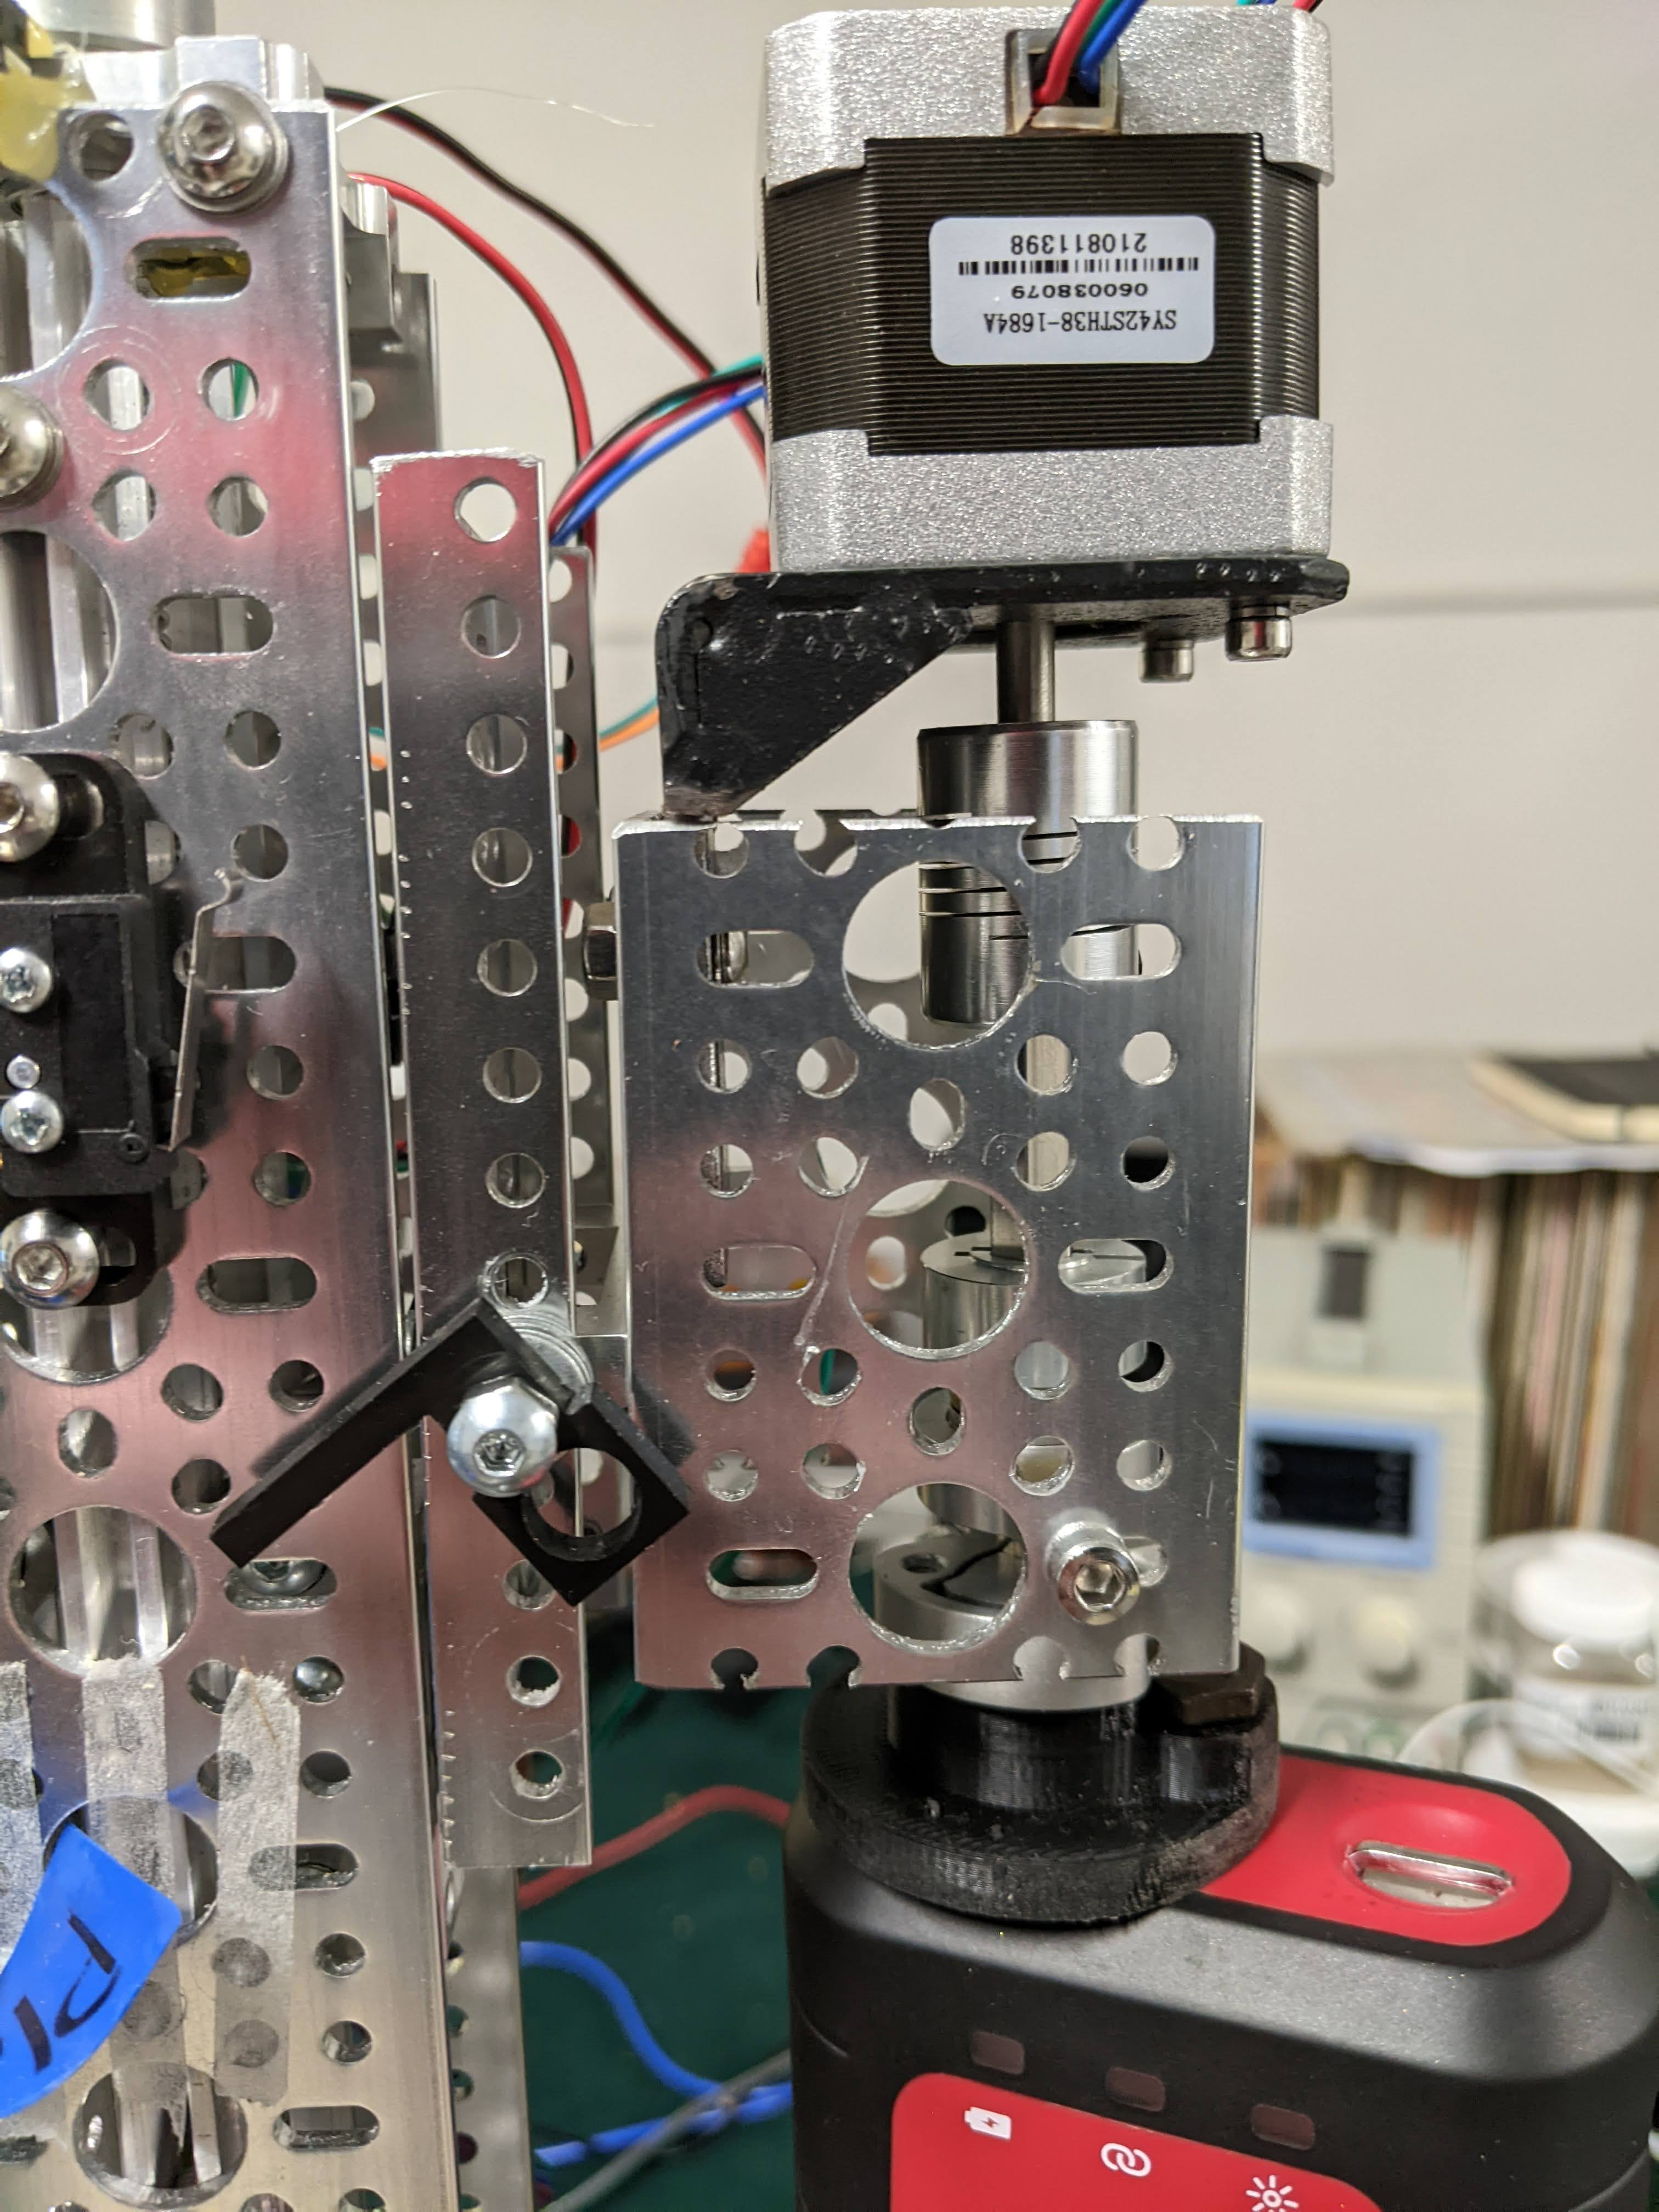
\includegraphics[width=0.9\textwidth]{VERT_MOVE_CARRIAGE.jpg}
	\caption{Instrument Carriage}
	\label{fig:Instrument Carriage}
\end{figure}
The figure *ref figure above* shows the updated carriage that supports the instrument, motor and limit switch trigger. It moves vertically via the rotation of a lead screw and is guided by rails on either side. It moves vertically by rotating the motor located at the bottom of the vertical structure.\\
The main difference between this and *ref original carriage design* is the position the HLR is held, when attached. This configuration better aligns the HLR with the sample container. \\
\begin{figure}[h]
	\centering
	\rule{0.5\textwidth}{0.5\textwidth}%\includegraphics[width=0.9\textwidth]{VERT_MOVE_MOTOR_MOUNT.jpg}
	\caption{Instrument Rotation Motor Mount}
	\label{fig:Instrument Rotation Motor Mount}
\end{figure}
The figure *ref figure above* shows the updated configuration for the instrument rotation motor. \\
This arrangement was partially forced by the relocation of the instrument but also removes complexity by eliminating the need for gears. \\
\begin{figure}[h]
	\centering
	\rule{0.5\textwidth}{0.5\textwidth}%\includegraphics[width=0.9\textwidth]{mechanical_design_modifications.jpg}
	\caption{Force Sensor to head of instrument}
	\label{fig:Force Sensor to head of instrument}
\end{figure}
The figure *ref figure above* shows the addition of a force sensor to the face of the instrument (glued onto the custom instrument head). \\
This allows the system to detect when the instrument has come into contact with the surface of the soil sample. \\
\begin{figure}[h]
	\centering
	\rule{0.5\textwidth}{0.5\textwidth}%\includegraphics[width=0.9\textwidth]{MANUAL_MOVE_TRIGGER_SWITCH.jpg}
	\caption{trigger manual movement}
	\label{fig:Manual Movement Trigger}
\end{figure}
*description of manual movement/orientation*\\
\textbf{other design notes}\\
The switches and triggers used within the system act both to allow the system to automatically orientate each motor but also add a layer of safety...*elaborate* \\
The way the program handles these inputs is described in *ref coding section* \\
%%%%%%%%%%%%%%%%%%%%%%%%%%%%%%%
\section{Final Program Design}\label{sec:Final Program Design}
This section presents the final program design for the project.\\
Add details hear!!!\\
\textbf{Subsections:}
\begin{itemize}
	\item Program Design and Implementation
	\item Instrument Movement Control
	\item Instrument Scan Control
	\item Data Collection
\end{itemize}

\subsection{Program Design and Implementation}\label{sub:Program Design and Implementation}
As can be seen in *ref schema/program design* there are 3 distinct programs that perform different operations, in order to achieve.... *ADD*. The design and role is explored below. \\
\begin{figure}[h]
	\centering
	\rule{0.5\textwidth}{0.5\textwidth}%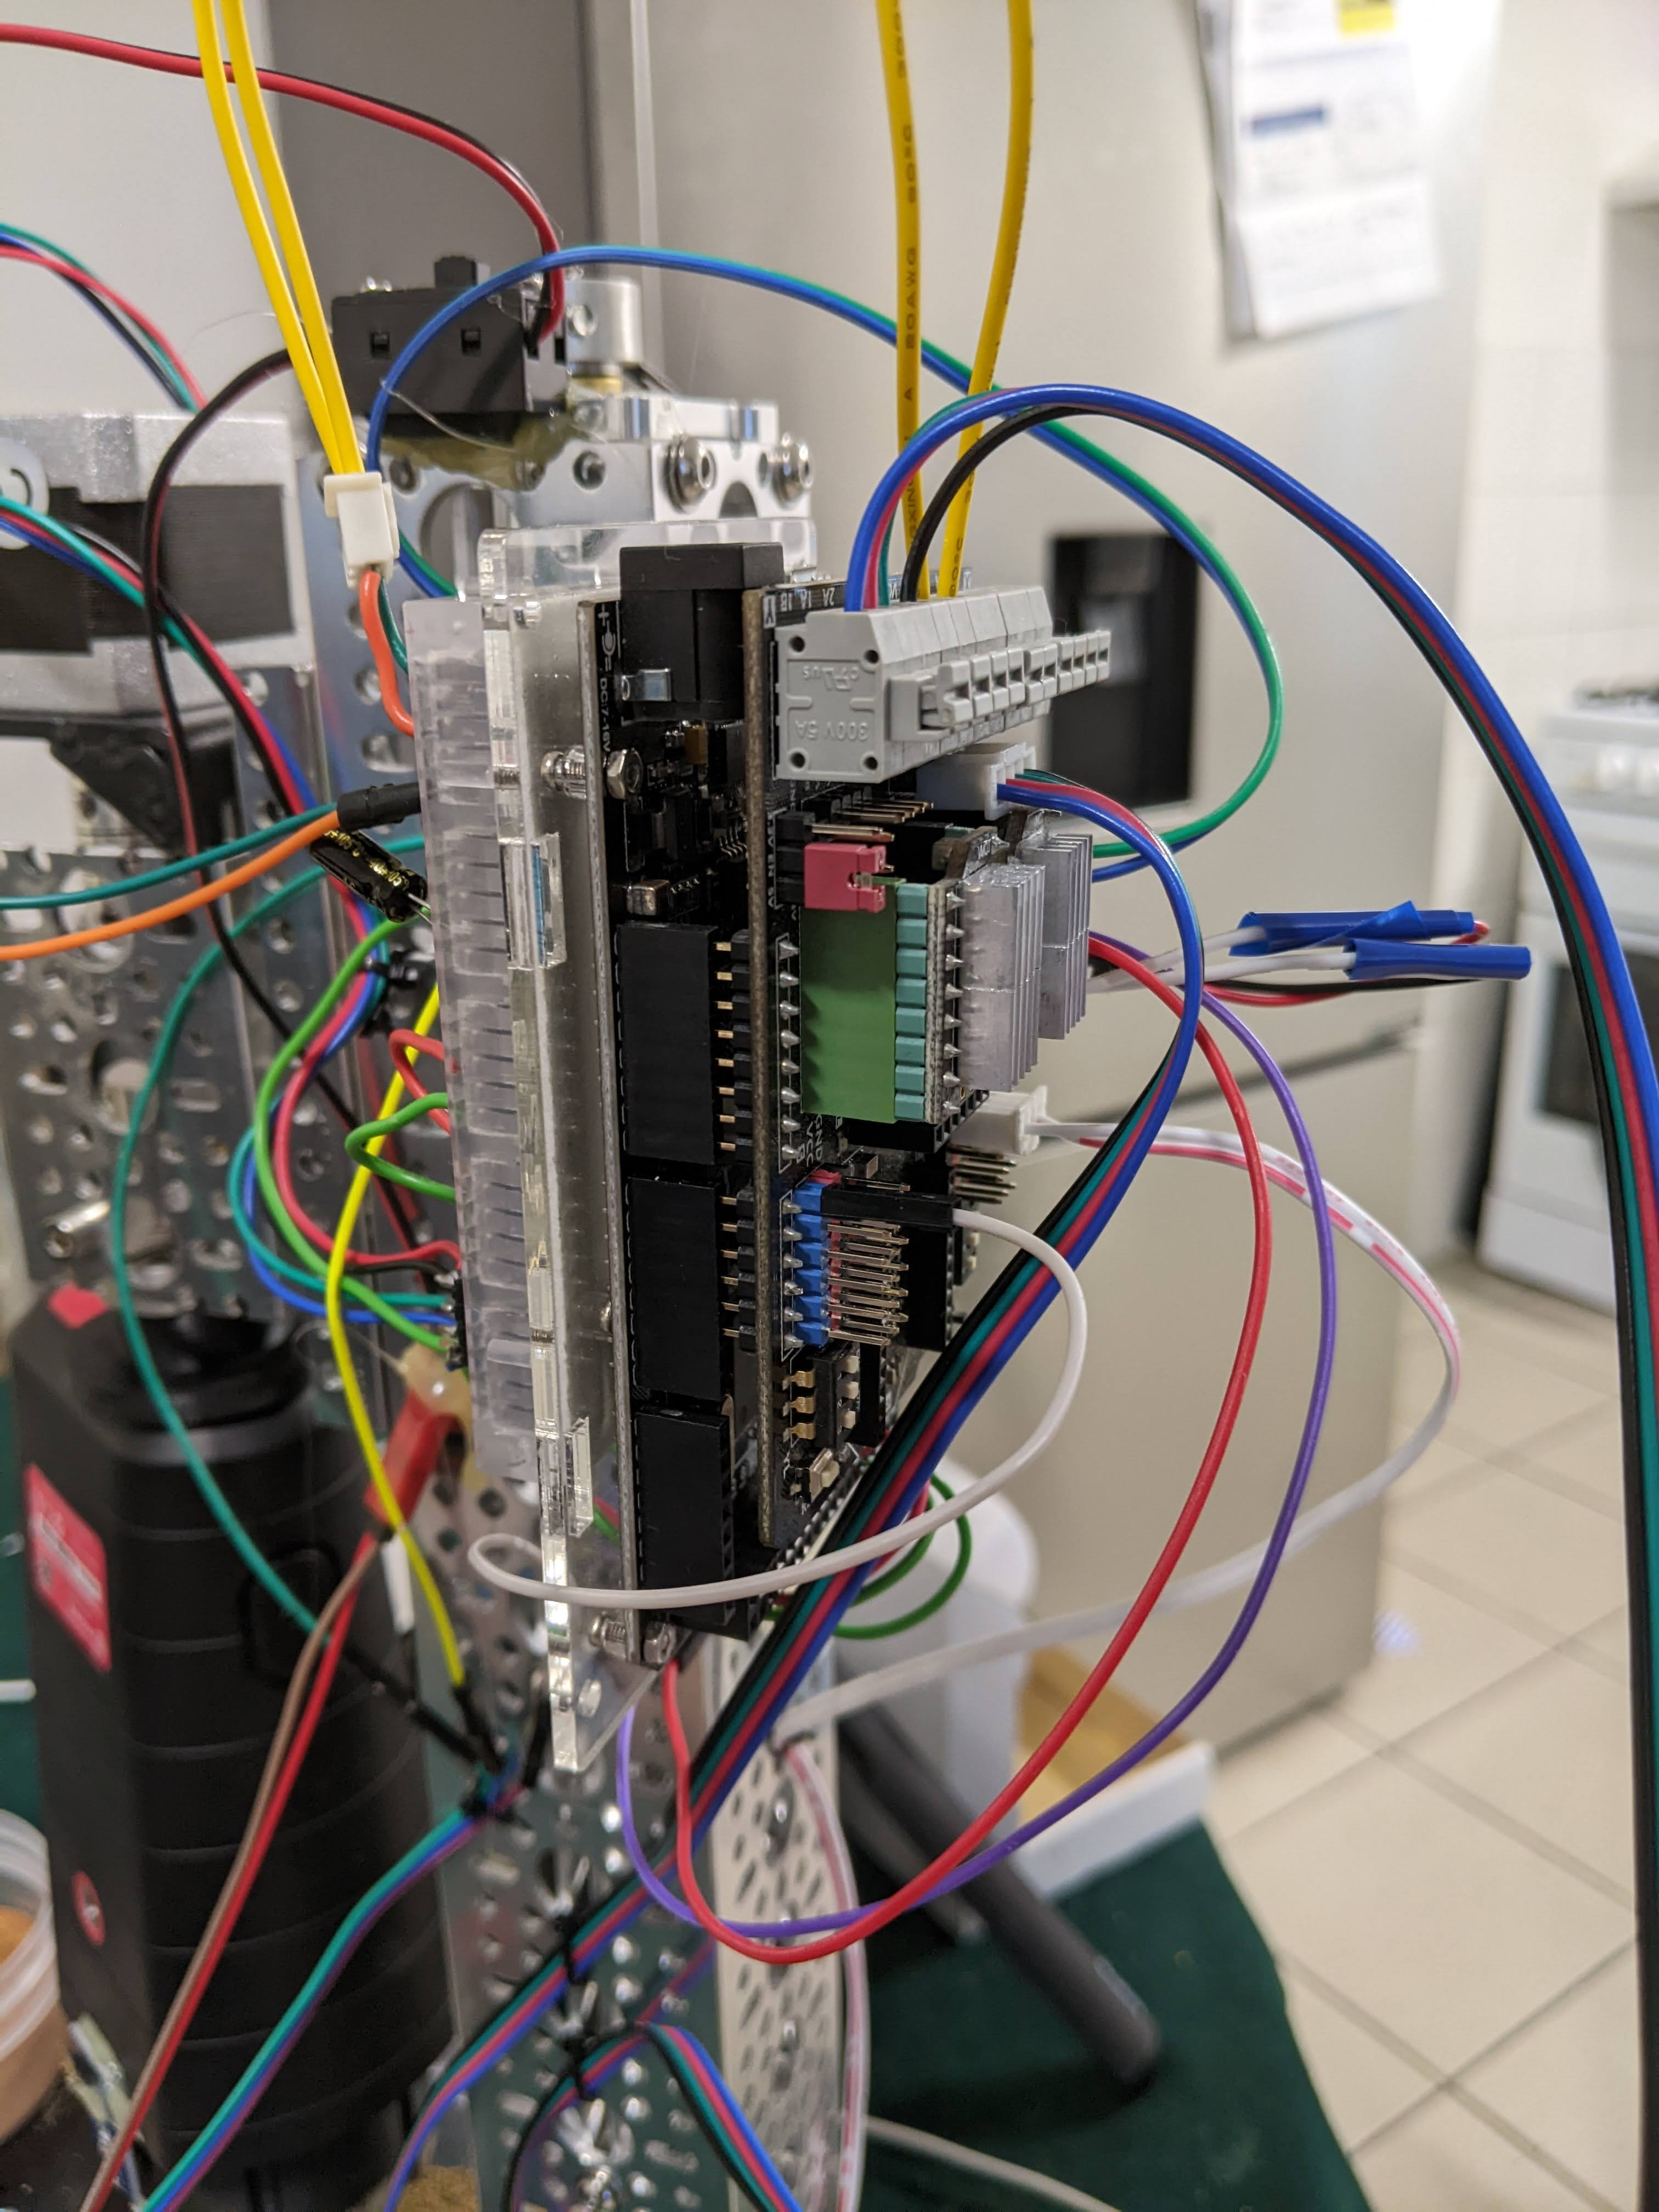
\includegraphics[width=0.9\textwidth]{ARDUINO_MOUNTED.png}
	\caption{Arduino Mounted In Place}
	\label{fig:Arduino Mounted In Place}
\end{figure}
Connected to the arduino is 3x motor controllers....*add details/references*. \\
\textbf{Motor Control Program - Big Mover}\\
All physical hardware (motors, switches etc) is controlled by an Arduino Mega 2560 running a custom program dubbed 'Big Mover'. Big Mover was setup to be easy to use by accepting integer inputs via serial communication (USB input with a PC) to switch states within a number of nested state machines. These state machines allows a user to navigate between options for running the program in different modes and perform setup routines.\\

Code snippets of the main program features can be found in *ref appendix for main menu code snippets* for more details on this program. \\
\begin{figure}[h]
	\centering
	\rule{0.5\textwidth}{0.5\textwidth}%\includegraphics[width=0.9\textwidth]{control_schema_implementation.png}
	\caption{Big Mover Program}
	\label{fig:Big Mover Program}
\end{figure}
Further details of this program are supplied in... *ADD REF* \\

\textbf{Human Machine Interface Program - Supervisor System}\\
This program was written in C Sharp to be run on any windows PC and acts as... \\
\begin{figure}[h]
	\centering
	\rule{0.5\textwidth}{0.5\textwidth}%\includegraphics[width=0.9\textwidth]{control_schema_implementation.png}
	\caption{Supervisor System}
	\label{fig:Supervisor System}
\end{figure}

\textbf{Instrument Control Program - HLR Desktop App}\\
This was provided by Hone Global as a basis for controlling the HLR.... \\
\begin{figure}[h]
	\centering
	\rule{0.5\textwidth}{0.5\textwidth}%\includegraphics[width=0.9\textwidth]{control_schema_implementation.png}
	\caption{HLR Desktop App}
	\label{fig:HLR Desktop App}
\end{figure}

Previous use.. \\

Edits... \\


\subsection{Instrument Movement Control}\label{sub:Instrument Movement Control}
This subsection details the specifics of controlling the Arduino and motors, both manually and through automatic routines. It includes screenshots of the menu structure for the Arduino program and describes the manual and automatic control functionalities. Additionally, it may include screenshots of commands/messages exchanged between the programs.	\\
\begin{itemize}
	\item Methods for each subsystem
	\item Menu Structure for Program Control
	\item 
	\item Pre-defined Movement routines
\end{itemize}
The figure below illustrates methods written for each subsystem to keep the program well organised and easy to read or edit.\\
Each method contains all functions required to control one of the motors. This separates the movement functions, as each motor has a separate function and will require it's own set of movement functions
\begin{figure}[h]
	\centering
	\rule{0.5\textwidth}{0.5\textwidth}%\includegraphics[width=0.9\textwidth]{menu_structure_manual_control.png}
	\caption{Methods for each subsystem}
	\label{fig:Methods for each subsystem}
\end{figure}
The figure below illustrates the menu structure for the main menu and scan control menu.\\
This enables a user to easily input the routine they want to run by inputting the corresponding integer into the serial monitor. This also enables autonomous routines to be run by parsing the necessary integer to the Arduino using a separate program... \\
\begin{figure}[h]
	\centering
	\rule{0.5\textwidth}{0.5\textwidth}%\includegraphics[width=0.9\textwidth]{menu_structure_manual_control.png}
	\caption{Menu Structure for Program Control}
	\label{fig:Menu Structure for Program Control}
\end{figure}
The figure below illustrates the some of the pre-defined Movement routines used throughout the program to control different movement routines...\\
\begin{figure}[h]
	\centering
	\rule{0.5\textwidth}{0.5\textwidth}%\includegraphics[width=0.9\textwidth]{menu_structure_manual_control.png}
	\caption{Pre-defined Movement routines}
	\label{fig:Pre-defined Movement routines}
\end{figure}

\subsection{Instrument Scan Control}\label{sub:Instrument Scan Control}
This subsection briefly explains the usage of the Hone desktop app and provides specific details on how the desktop program sends information and controls the instrument. A screenshot of the app can be included if necessary.	\\

\textbf{Instrument Scan Control}
% Quick explanation/summary of using the Hone Desktop app
% Screenshot of app (maybe)
% Detail specifics of how the C# program sends info/controls the instrument

\begin{itemize}
	\item 
	\item 
	\item 
\end{itemize}
The figure below shows the Hone desktop app used for instrument scan control.\\
\begin{figure}[h]
	\centering
	\rule{0.5\textwidth}{0.5\textwidth}%\includegraphics[width=0.9\textwidth]{hone_desktop_app.png}
	\caption{Hone Desktop App}
	\label{fig:Hone Desktop App}
\end{figure}


%%%%%%%%%%%%%%%%%%%%%%%%%%%%%%%Data Collection
\subsection{Data Collection}\label{sub:Data Collection}
This subsection briefly explains the usage of the Hone desktop app and provides specific details on how the desktop program sends information and controls the instrument. A screenshot of the app can be included if necessary.	\\

\textbf{Data Collection}
The figure below shows an example of meta data that was sent to the Hone Desktop App. then saved... \\
\begin{figure}[h]
	\centering
	\rule{0.5\textwidth}{0.5\textwidth}%\includegraphics[width=0.9\textwidth]{hone_desktop_app.png}
	\caption{Parsing Meta Data}
	\label{fig:Parsing Meta Data}
\end{figure}
The figure below shows an example of a captured scan being displayed as a line graph....
\begin{figure}[h]
	\centering
	\rule{0.5\textwidth}{0.5\textwidth}%\includegraphics[width=0.9\textwidth]{hone_desktop_app.png}
	\caption{Scan Data}
	\label{fig:Scan Data}
\end{figure}
%%%%%%%%%%%%%%%%%%%%%%%%%%%%%%%Data Collection
\newpage
\section{Final Mechanical Design}\label{sec:Final Mechanical Design}
% summary of the section
\textbf{Subsections:}\\
\begin{itemize}
	\item Design Features
	\item Design Justifications
	\item Testing
	\item Data Collection
\end{itemize}

\subsection{Design Features}\label{sub:Design Features}
This subsection describes the features of the final mechanical design. It may include details on the prototype build, adjustments made, and any additional features incorporated.\\
% Need to figure this out...

\begin{itemize}
	\item Feature 1
	\item Feature 2
	\item Feature 3
\end{itemize}
\textbf{Prototype Build}\\

The figure below showcases the adjusted prototype build of the system.
\begin{figure}[h]
	\centering
	\rule{0.5\textwidth}{0.5\textwidth}%\includegraphics[width=0.9\textwidth]{prototype_build_adjustments.jpg}
	\caption{Adjusted Prototype Build}
	\label{fig:Adjusted Prototype Build}
\end{figure}

\subsection{Design Justifications}\label{sub:Design Justifications}
This subsection covers the fine-tuning process of the mechanical design. It may discuss the optimization of components, alignment adjustments, and any other refinements made.\\

\begin{itemize}
	\item 
	\item 
	\item 
\end{itemize}
%%%%%%%%%%%%%%%%%%%%%%%%%%%%%%%
\newpage
\section{System Testing}\label{sec:System Testing}
% summary of section
\textbf{Subsections:}\\
\begin{itemize}
	\item Movement Testing
	\item Data Collection Tests
	\item Testing Assessment
\end{itemize}
\subsection{Movement Tests}\label{sub:Movement Tests}
This subsection describes the movement tests conducted on the system. It includes timed tests moving to various positions and provides relevant photos documenting the tests.\\
*FILL in with summary of tests that will be performed*\\
\subsubsection{Movement Test 1 - Repeated Single Sample Scanning}\label{subsub:Movement Test 1}
\textbf{Hypothesis/Expected Outcome}\\

The system will move the instrument up and down between the 'wait' and 'scan' position 5 times, at a speed that matches or exceeds the same movement repeated by a human.\\

\textbf{Test Preparation}\\

The system was setup to complete the movement routine and trigger a scan, without saving the data.\\
As the data collection will be tested separately, *shown in section... ref* it is assumed that captured data...\\ 
This allowed focus to be paid to timing the movement routine and monitoring the system for correct motor control. \\

\textbf{Test Control}\\
A single sample was scanned 5 times, controlling the instrument by hand.\\
Again, this data was not saved so more attention could be paid to timing the movement routine, while managing the instrument. \\

\textbf{Test Results}\\

Control Time:  \\
Automated Routine Time:  2 Minutes 45 Seconds\\

\textbf{Documentation/Media}\\

The figure below captures the system during one of the movement tests.\\

\begin{figure}[h]
	\centering
	\rule{0.5\textwidth}{0.5\textwidth}%\includegraphics[width=0.9\textwidth]{movement_test_1.jpg}
	\caption{System Movement Test 1}
	\label{fig:System Movement Test 1}
\end{figure}

Additionally, a video recording of the movement test is available at the following link: [insert link to video].\\

\subsubsection{Movement Test 2 - Multi Sample Scanning}\label{subsub:Movement Test 2}
\textbf{Hypothesis/Expected Outcome}

The hypothesis for this test is that the system will accurately move to a series of predetermined positions in a coordinated sequence.\\

\textbf{Test Preparation}\\

The test was prepared by defining the specific positions and the sequence in which the system should move. The necessary commands were programmed into the control software.\\

\textbf{Test Control}\\

The test was controlled by initiating the sequence of movements through the control program. The program communicated the movement commands to the microcontrollers, which executed the movements in the predetermined sequence.\\

\textbf{Test Results}\\

The test results showed that the system successfully performed the coordinated sequence of movements, accurately moving to each predetermined position in the specified order.\\

\textbf{Documentation/Media}\\

The figure below captures the system during one of the movement tests.\\
This test involved scanning 5 different samples, loaded into the sample plate, once. \\

\begin{figure}[h]
	\centering
	\includegraphics[width=0.9\textwidth]{SINGLE_SCAN_5_SAMPLES.jpg}
	\caption{System Movement Test 2}
	\label{fig:System Movement Test 2}
\end{figure}

A video recording of the movement test is available at the following link: [insert link to video].\\

\subsubsection{Movement Test 3}\label{subsub:Movement Test 3}
\textbf{Hypothesis/Expected Outcome}\\

The hypothesis for this test is that the system will accurately move to specific positions while maintaining stability and without any unintended oscillations.\\

\textbf{Test Preparation}\\

The test was prepared by selecting a set of positions at different locations within the system's range of motion. These positions were chosen to test the stability and accuracy of the system.\\

\textbf{Test Control}\\

The test was controlled by sending movement commands to the system to move to the specified positions. The commands were executed through the control program, which communicated with the microcontrollers responsible for motor control.\\

\textbf{Test Results}\\

The test results demonstrated that the system successfully moved to the specified positions with stability and accuracy. There were no unintended oscillations or instability observed during the movements.\\

\textbf{Documentation/Media}\\

The figure below captures the system during one of the movement tests.\\

\begin{figure}[h]
	\centering
	\rule{0.5\textwidth}{0.5\textwidth}%\includegraphics[width=0.9\textwidth]{movement_test_3.jpg}
	\caption{System Movement Test 3}
	\label{fig:System Movement Test 3}
\end{figure}

\subsection{Data Collection Tests}\label{sub:Data Collection Tests}
This subsection discusses the data collection tests performed on the system. It describes the various ways data was collected, such as spaced scanning, and provides relevant details and observations. Photos or screenshots of the testing setup can be included.\\

\subsubsection{Data Collection Test 1 - Data Collection Reliability}\label{subsub:Data Collection Test 1}
\textbf{Hypothesis/Expected Outcome}\\

The data collection test involved performing spaced scanning using the system. The goal was to collect data from different positions within the sample container and assess the system's ability to accurately capture measurements.\\
\textbf{Test Preparation}\\

\textbf{Test Control}\\

One of the reference samples supplied by Hone, was replaced with a random soil sample and labeled 'Control Soil', to act as a control for data management. \\
The spectral output of the Hone samples appear visually similar when viewed on a graph so the random soil sample was included to provide a distinctly different spectral output. When adding the Control Soil to the sample list, it performed double duty by ensuring output is not faked within the video and checking data in terms of the correct sample named being saved along side the spectral data. By being visually different, it is easy to identify if the spectral data is saved with the incorrect sample name. \\
\begin{figure}[h]
	\centering
	\rule{0.5\textwidth}{0.5\textwidth}%\includegraphics[width=0.9\textwidth]{data_collection_test_1.png}
	\caption{Data Collection Test Control - Control Soil Sample}
	\label{fig:Control Soil Sample}
\end{figure}
\textbf{Test Results}\\

The test results indicated that the system successfully performed spaced scanning and collected data from different positions within the sample container. The collected data showed consistent and accurate measurements.\\

\textbf{Other Observations}\\

The time taken to collect this data was...\\

Compared to doing it by hand...\\

\textbf{Documentation/Media}\\

The figure below showcases the data collection setup used during the tests.\\

\begin{figure}[h]
	\centering
	\rule{0.5\textwidth}{0.5\textwidth}%\includegraphics[width=0.9\textwidth]{data_collection_test_1.png}
	\caption{Data Collection Setup - Spaced Scanning}
	\label{fig:Data Collection Setup - Spaced Scanning}
\end{figure}

\subsubsection{Data Collection Test 2 - Scanning With Gap}\label{subsub:Data Collection Test 2}
When being used by hand, the instrument lens comes in contact with the surface of the soil, as the instrument is placed in the container. It is known that for the best quality scan, the lens should be place directly on the sample but this also means cleaning the lens between every sample that is scanned and increases the risk of cross contamination between samples. It is theorized that bringing the instrument lens within 5mm of the surface of the sample would allow sufficient scan quality, while keeping the lens clean. \\
In this data collection test, the system was set to position the instrument above the samples with a 4-5mm and the routine involved scanning 5 samples in sequence, automatically.\\ 
\textbf{Hypothesis/Expected Outcome}\\
A scan of sufficient quality may be taken, without the instrument lens touching the surface of the soil. \\
\textbf{Test Preparation}\\
\begin{enumerate}
	\item Adjust height of soil samples to be within 1mm (within container).
	\item Compress soil samples lightly.
	\item Orientate system to set the scanning position to 2-3mm above the surface of the soil samples.
	\item Take a background scan before beginning the scan routine. 
\end{enumerate}
\textbf{Test Control}\\
Sample spectra will be compared against spectra captured while the lens of the instrument is in contact with the surface of the sample. \\
\textbf{Test Results}\\
The figures below show the spectra captured during the test with...\\
\begin{figure}[h]
	\centering
	\includegraphics[width=0.9\textwidth]{Multi_Sample_Spectral_Data.png}
	\caption{Multi Sample Spectral Data}
	\label{fig:Multi Sample Spectral Data}
\end{figure}
\begin{figure}[h]
	\centering
	\rule{0.5\textwidth}{0.5\textwidth}%\includegraphics[width=0.9\textwidth]{Multi_Sample_Spectral_Data.png}
	\caption{Multi Sample Spectral Data}
	\label{fig:Test Control Data}
\end{figure}\\
\textbf{Other Observations}\\

The time taken to collect this data was...\\

Compared to doing it by hand...\\
\textbf{Documentation/Media}

No additional media or screenshots were captured for this specific test.\\

\subsection{Testing Assessment}\label{sub:Testing Assessment}
This subsection assesses the testing outcomes and compares them with the scope requirements. It highlights the achievements and areas that may require further attention or improvement.\\

\subsubsection{Movement Test Assessment}\label{subsub:Movement Test Assessment}
The movement tests conducted in Section \ref{sub:Movement Tests} were assessed to evaluate their outcomes in comparison to the hypothesis and expected outcomes.\\

\textbf{Movement Test 1}

The system's movement test 1 demonstrated successful movement to the desired positions within the specified time frame, aligning the sample tray and HLR as expected.\\

\textbf{Movement Test 2}

The system's movement test 2 successfully performed the coordinated sequence of movements, accurately moving to each predetermined position in the specified order.\\

\textbf{Movement Test 3}

The system's movement test 3 accurately moved to specific positions while maintaining stability and without any unintended oscillations.\\

\subsubsection{Data Collection Test Assessment}\label{subsub:Data Collection Test Assessment}
The data collection tests performed in Section \ref{sub:Data Collection Tests} were assessed to evaluate their outcomes in comparison to the hypothesis and expected outcomes.\\

\textbf{Data Collection Test 1}

The spaced scanning data collection test demonstrated the system's ability to collect data from different positions within the sample container with consistent and accurate measurements.\\

\textbf{Data Collection Test 2}

The continuous scanning data collection test showed that the system could collect data continuously as it moved through the sample container, producing smooth transitions between measurement points.\\
%%%%%%%%%%%%%%%%%%%%%%%%%%%%%%%
\newpage
\section{System Refinement}\label{sec:System Refinement}
\subsection{Issues Present in Testing}\label{sub:Issues Present in Testing}
This subsection documents the issues encountered during testing. It provides a summary of the parts that did and did not work as expected.

\subsection{Design Flaws}\label{sub:Design Flaws}
This subsection evaluates the design flaws identified in the system. It categorizes the flaws and assesses their severity. Relevant photos can be included.
% assess issues and categorize as flaws
% include 'severity' of flaw
% photos

\begin{itemize}
	\item 
	\item 
	\item 
\end{itemize}
\subsection{Proposed Fixes}\label{sub:Proposed Fixes}
This subsection presents proposed solutions for fixing the identified design flaws. It provides ideas and recommendations for addressing the flaws and improving the system's performance.
% Detail ideas for fixing the flaws present in the system 

\begin{itemize}
	\item 
	\item 
	\item 
\end{itemize}
%%%%%%%%%%%%%%%%%%%%%%%%%%%%%%%
\newpage
\section{Critical Analysis of Position}\label{sec:Critical Analysis of Position}
\subsection{Scope Requirement Fulfillment}\label{sub:Scope Requirement Fulfillment}
This subsection offers a final comparison between the scope requirements and the achieved outcomes. It evaluates the extent to which the project has fulfilled the initial scope.

\subsection{Final System Assessment}\label{sub:Final System Assessment}
This subsection provides a comprehensive assessment of the final system. It analyzes the system's strengths, weaknesses, and overall performance in relation to the project goals.

\subsection{Conclusions Gained From Testing}\label{sub:Conclusions Gained From Testing}
This subsection discusses the conclusions drawn from the testing phase. It highlights any significant findings or insights gained through experimentation.\\
%%%%%%%%%%%%%%%%%%%%%%%%%%%%%%%
\newpage
\section{Conclusion}\label{sec:Conclusion}
This section concludes the report, summarizing the overall progress and outcomes of the project. It reflects on the initial goals, achievements, challenges faced, and lessons learned throughout the development process.

\textbf{Subsections:}\\
\begin{itemize}
	\item Project Summary
	\item Critical Review of Objectives
	\item Critical Analysis of the Approach
\end{itemize}

\subsection{Project Summary}\label{sub:Project Summary}
% Summary of the project as a whole
\begin{itemize}
	\item 
	\item 
	\item 
\end{itemize}

\subsection{Critical Review of Objectives}\label{sub:Critical Review of Objectives}
% Summary of objectives and their status
\begin{itemize}
	\item 
	\item 
	\item 
\end{itemize}

\subsection{Critical Analysis of the Approach}\label{sub:Critical Analysis of the Approach}
% Reflection on the approach taken throughout the project
\begin{itemize}
	\item 
	\item 
	\item 
\end{itemize}
%%%%%%%%%%%%%%%%%%%%%%%%%%%%%%%
\newpage
\bibliography{references} % call to references.bib
\bibliographystyle{harvard} % call to harvard.bst
% Add the \cite{} commands for each website reference
\cite{website1}
\cite{website2}
\cite{website3}
\cite{website4}
\cite{website5}
\cite{website6}
\cite{website7}
\cite{website8}
\cite{website9}
\cite{website10}
%%%%%%%%%%%%%%%%%%%%%%%%%%%%%%%
\newpage
\section{Acknowledgments}\label{sec:Acknowledgments}
% Acknowledge any individuals or organizations that contributed to the project
I would like to express my sincere gratitude to the following individuals and organizations for their invaluable contributions and support throughout the project:\\

\begin{enumerate}
	\item Person 1: Acknowledgement statement 1.
	\item Person 2: Acknowledgement statement 2.
	\item Person 3: Acknowledgement statement 3.
\end{enumerate}

\appendix
\newpage

\section{Appendix A - Reflection}\label{app:Reflection}
Reflect...\\

\newpage
\section{Appendix B - Program Scripts}\label{app:Program Scripts}

\subsection{Appendix B.1 - Script 1}\label{subapp:Script 1}
% Include the content of Script 1 here

\subsection{Appendix B.2 - Script 2}\label{subapp:Script 2}
% Include the content of Script 2 here

\subsection{Appendix B.3 - Script 3}\label{subapp:Script 3}
% Include the content of Script 3 here

\newpage
\section{Appendix C - Spectral Data}\label{app:Spectral Data}

\subsection{Appendix C.1 - Spectral Data 1}\label{subapp:Spectral Data 1}
% Include the content of Spectral Data 1 here

\subsection{Appendix C.2 - Spectral Data 2}\label{subapp:Spectral Data 2}
% Include the content of Spectral Data 2 here

\subsection{Appendix C.3 - Spectral Data 3}\label{subapp:Spectral Data 3}
% Include the content of Spectral Data 3 here

\newpage
\section{Appendix D - Mechanical Design Details}\label{app:Mechanical Design Details}
% Include the mechanical design details here

\end{document}
